% Use class option [extendedabs] to prepare the 1-page extended abstract.
\documentclass[extendedabs]{bmvc2k}
\usepackage[colorlinks = true,
            linkcolor = blue,
            urlcolor  = blue,
            citecolor = blue,
            anchorcolor = blue]{hyperref}
\usepackage{kotex} % 한국어 사용 가능

% Document starts here
\begin{document}
\title{pix2pix and cycle GAN }
\addauthor{
Lee Gwan Hui$^1$, \today}{}{1}
\addinstitution{
$^1$2017142136, Department of Electrical and Electronic Engineering, Yonsei University.}
\maketitle
\let\thefootnote\relax\footnote{This is an extended abstract. The full paper is available at the \href{https://github.com/LeeGwanHui/TIL/tree/main/deeplearning_ham}{github}. }
\vspace{-0.2in}

\section{pix2pix\cite{isola2017image}}
 \subsection{motivation}
  \quad 저자들은 image-to-image translation task를 위해 conditional adversarial networks을 연구했다. conditional adversarial networks는 input image를 output image로 
  mapping 시키는 것을 학습할 뿐만 아니라 이 mapping을 학습하기 위한 loss function을 학습한다. 기존의 연구들은 image-to-image domain 마다 loss function 혹은 model을 짜야 했었는데 
  이 연구는 same generic approach이 가능하다. 제시하는 모델은 다양한 task에 적용가능하고 또한 parameter을 일일히 찾지 않아도 되는 편리성을 가지고 있다. 
  즉, 정리하자면 기존의 연구는 task 마다 mapping function과 loss function을 변경해주었어야 하는데 이 연구에서 이를 공통으로 해결하는 모델을 제시한 것이다.
  이 논문에서는 cGAN을 이용해서 첫번째로 다양한 문제에 적용가능토록하였고 두번째로 간단하지만 result가 좋은 framework를 제시한다는 기여점이 있다.

 \subsection{model의 형태\cite{youtube}}
 \quad 기존의 CNN의 경우 blurry result을 생산해낸다는 단점이 있었는데 GAN 모델을 사용하면 blurry result는 fake로 학습될 것이기 때문에 비교적 선명한 이미지를 얻을 수 있다.  
 이 논문에서는 cGAN을 사용했는데 cGAN이란 noise vector 뿐만 아니라 input image x 도 넣어서 그 이미지를 기본으로 원하는 분포의 domain으로 변화시키는데 이용된다. 즉, 
 conditional GANs의 경우에는 observed image x와 random noise vector z로 부터 y로 mapping 되는 것을 배운다.
 conditional GAN은 아래와 같이 표현할 수 있다.
 $$ L_{cGAN}(G,D) = E_{x,y} [ log D(x,y) ] + E_{x,z} [log(1-D(x,G(x,z)))]$$
 $$G^* = argmin_G max_D L_{cGAN}(G,D) $$
 GAN은 아래와 같이 표현할 수 있다.
 $$ L_{GAN}(G,D) = E_y[log D(y)] + E_{x,z}[log(1-D(G(x,z)))]$$
 두개의 차이점을 살펴보자면 cGAN의 경우에는 input x을 D에도 사용한다는 점이다.
 기존의 연구의 경우 L2 distance loss를 사용하였지만 이 연구에서는 blurring이 좀 덜한 L1 distance를 사용할 것이다. 
 \newline  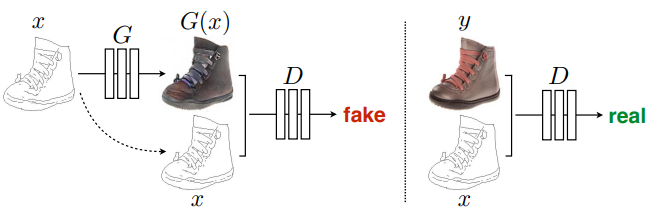
\includegraphics[width=8cm]{images/00_pix2pix.PNG}
 \newline 이 연구의 최종  objective는 이래와 같다. L1 loss를 사용할 수 있는 이유는 실제 정답이 되는 데이터 쌍을 가지고 있기 때문이다.
 고로 아래 목적함수에서 첫항은 현실적인 이미지를 만드는 loss이고 2번째항은 실제 정답과 유사하도록 학습하는 항이다.
 $$ G^{*} = argmin_G max_G min_D L_{cGAN}(G,D) + \lambda L_{L1}(G)$$
 $$ L_{L1}(G) = E_{x,y,z}[||y-G(x,z)||_1] $$
 이 연구에서 제시하는 모델은 z없이 x로부터 y로 mapping이 가능하지만 deterministic output을 생산한다는 단점이 있다.
 그래서 stochastic output을 생산해내고 전체 entropy을 capture 위한 cGAN을 design은 매우 중요하고 아직 남겨진 문제이다.
 이 논문 전에 기본적은 img2img problem은 encoder-decoder 형태로 설계되는 것이 대부분이었다. 이 방법을 사용할 경우 생성된 이미지가 
 실제와는 다르다는 것을 파악한 저자들은 U-Net 구조를 사용하였다. U-Net 구조는 skip connection을 사용하는 모델로 skip connection이란
 CNN을 많이 통과하면 더 높은 high feature을 뽑아내지만 위치정보를 잃는다는 아이디어에서 착안한 것으로 concatenate 을 이용해서 앞단의 정보를 유지하고
 CNN을 더 통과한 feature도 같이 사용하면서 의미있는 결과를 만들어낸다.
 \newline  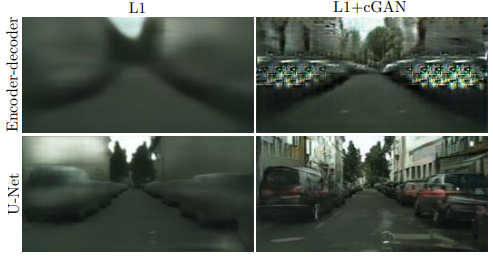
\includegraphics[width=8cm]{images/01_pix2pix.PNG}
 \newline 이 외에도 이 논문에서는 patchGAN을 이용하였다. Patch cGAN이란
 NxN의 전체 이미지중 일부가 real인지 fake인지 판단하는 것이다. PatchGAN의 경우 더 적은 parameter로 구성되어 있고 더 빠르며 더 큰 이미지 크기에도 적용가능하다.
 
 \subsection{Experiments}
 \quad 이 논문에서는 실험의 성능 평가로 두가지 방법을 사용했다. 하나는 AMT(Amazon Mechanical Turk) 로 사람이 생성된 이미지가 의미있다고 생각하는지를 
 판단하는 지표와 두번째는 FCN-score을 사용했는데 FCN은 segmentation에서 배운 semantic classifier이다. 생성된 이미지가 정말로 현실적이라면 classifier도
 생성된 이미지를 classify할 수 있을거라는 아이디어에서 측정한 지표이다. 
 \newline  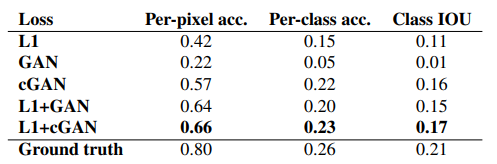
\includegraphics[width=6cm]{images/02_pix2pix.PNG}
 \newline 위의 결과는 다른 loss를 사용했을 때 어떤 것이 ground truth와 가장 유사한지를 보여준다. 이 경우 L1과 conditional GAN을 함께 사용한 loss가 가장 유사함을 보여준다.
 \newline  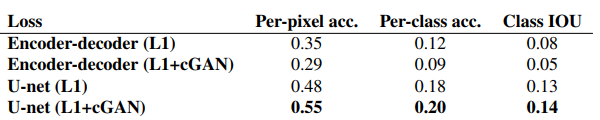
\includegraphics[width=6cm]{images/03_pix2pix.PNG}
 \newline 위의 결과는 다른 generator 구조를 착안했을 때 label에서 photo를 만들때의 score을 평가한 것이다. U-net의 구조가 encoder-decoder의 구조보다 더 정확성이 높음을 볼 수 있다.
 \newline  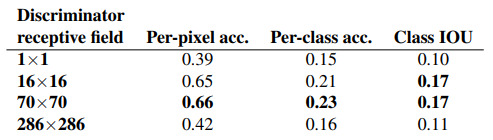
\includegraphics[width=6cm]{images/04_pix2pix.PNG}
 \newline 위의 결과는 patch size별로 정확도를 나타낸다. 70x70가 가장 정확도가 높아 PatchGAN을 사용할때 70x70을 사용할 것이다. 참고로 전체 이미지는 256x256 이미지이다. 


 \subsection{Conclusion}
 \quad 이 논문에서는 conditional GAN으로 다양한 image-to-image translation task에 적용해보고 좋은 graphical output을 얻을 수 있었다.
 이 network의 특징으로는 task와 data에 연관된 loss를 자동적으로 배운다는 점에 있다. 이 논문의 한계로는 학습시킬 때 서로 다른 두 domain의 X,Y의 데이터를 한쌍으로 학습시킨다는 점이다.
 한쌍으로 묶이지 않는 dataset에서는 적용이 불가능하다는 단점 뿐만 아니라 한쌍으로 묶기 위한 기초작업에 시간과 돈이 필요하다는 단점이 있다. 
 여기서 말하는 한쌍의 데이터를 의미하는 것은 예를 들면 실제 구두 사진과 그 구두를 스케치한 사진이 각각 Y,X로 짝이 지어짐을 말한다. 

\section{cycle GAN\cite{zhu2017unpaired}}
 \subsection{motivation}
 \quad 위의 논문 Pix2Pix의 경우 paired dataset에서 진행해야 한다는 단점이 있다. 즉 paired data를 만들어야 하는데 이 작업이 가능한 task가 있는 반면
 비용이 많이 들고 혹은 그냥 말을 얼룩말로 바꾸는 것처럼 까다로운 경우도 있다. 그렇기 때문에 이미지 별로 matching 되기 보다는 실제 사진, 
 그림처럼 domain으로 매칭되는 unpaired dataset을 학습하는 방법이 있을까하는 고민에서 고안하였다.
 
 \subsection{model의 형태\cite{youtube_cycle}}
 \quad 이 저자들은 paired input-output examples이 없이 domain 사이를 translate하는 algorithm을 제안한다. 이를 위해 필요한 가정이 domain 사이의 근본적인 관계가 
 있다는 것이다. 모델의 전체적인 학습과정은 G를 학습시켜서 $\hat{y} = G(x)$ 를 구하는데 이는 image y $\in$ Y 와 구별할 수 없도록 학습시켜야 한다.
 목적은 output distribution over $\hat{y}$ 와 실제의 분포인 $p_{data}(y)$ 를 match되도록 하는 것이다. optimal G의 경우 domain X에서 Y와 같도록 분포된 domain $\hat{Y}$ 로 translate 시켜준다.
 그러나 이러한 변환은 개별 입력 x와 출력이 의미 있는 방식으로 쌍을 이루는 것을 보장 못할 뿐더러 또한 실제로, 적대적인 목표를 단독으로 최적화하는 것이 어렵다.
 즉 mode collapse 문제가 발생한다. 이 문제를 해결하기 위해서 저자들은 “cycle consistent”을 도입했다. 이는 정방향 뿐만 아니라 역방향도 학습시키는 것으로
 translator G : X → Y 와 translator F : Y → X 를 모두 학습시켜 일대일 대응으로 만드는 것이다. 또한 F(G(x)) ≈ x 과 G(F(y)) ≈ y 되도록 하는 cycle consistency loss를 사용한다.
 모델을 조금 더 자세히 살펴보자면 adversarial loss를 적용했다.
 $$ L_{GAN}(G,D_Y,X,Y) = E_{y~p_{data}(y)}[log D_y(y)] + E_{x~p_{data}(x)}[log(1-D_Y(G(x)))] $$
 하지만 위의 GAN의 loss 홀로는 input $x_{i}$ 로부터 바라는 output $y_{i}$을 생성한다는 보장이 없다. 즉 x의 content를 유지한 상태로 output을 만든다는 보장이 없다는 것이다.
 즉 매칭되는 output y없이 단순히 x를 target domain Y로 바꾸어서 입력의 정보에 관계없이 Y domain에 해당하는 output을 낼 수 있다는 것이다. 추가적인 제약 조건이 반드시 필요하다는 것을 알 수 있다.
 그래서 $ x \rightarrow G(x) \rightarrow F(G(x)) \approx x $ 가 가능한 forward cycle consistency를 고려하고 비슷하게 $ y \rightarrow F(y) \rightarrow G(F(y)) \approx y $ 
 가 가능한 backward cycle consistency를 고려할 것이다. 그래서 loss를 새로 만들어주면 아래와 같다.
 $$ L{cyc}(G,F) = E_{x ~ p_{data}(x)}[||F(G(x)) = x||_1] + E_{y~p_{data}(y)}[||G(F(y))-y||_1] $$
 위에서 1이 의미하는 것은 L1 norm을 사용한다는 것이다. 위의 핵심은 G(x)가 원본 이미지로 다시 돌아갈 수 있도록 하는 것이다. 
 \newline  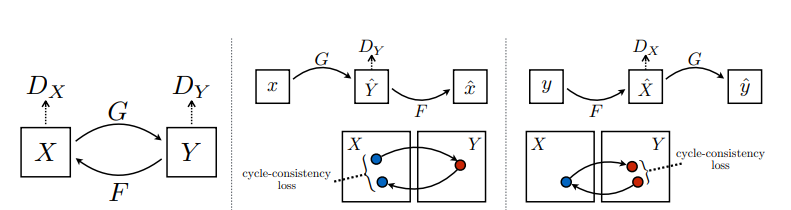
\includegraphics[width=\linewidth]{images/05_cycleGAN.PNG}
 \newline 위의 그림을 보면 알 수 있듯이 학습을 시킬때 cycle consistency loss를 이용해서 다시 복구될 수 있도록 학습을 진행한다는 것이다.
 이 때 G와 F는 역함수의 관계에 있다. 전체적인 objective function은 아래와 같다.
 $$ L(G,F,D_X,D_Y) = L_{GAN}(G,D_Y,X,Y) + L_{GAN}(F,D_X,Y,X) + \lambda L_{cyc}(G,F) $$
 GAN loss의 첫째항은 G가 만든 이미지가 domain Y에 근접하게 만드는 것이고 두번째항은 F가 만든 이미지가 domain X에 다가가도록 
 마지막 항은 두 함수가 autoencoder로 이용할 수 있도록 학습되는 항으로 X domain에서 Y domain으로 서로 1대1 대응이 되도록 학습하는 것을 목표로 한다.
 얻고자 하는 G와 F는 아래와 같다.
 $$ G^*, F^* =argmin_{G,F} max{D_x,D_Y} L(G,F,D_X,D_Y) $$
 실제 모델의 architecture의 경우에는 70x70 PatchGAN을 사용하고 세개의 convolutions와 residual block, 두개의 fractionally -strided convolutions 를 사용한다. 
 또한 한개의 convolution으로 RGB로 mapping되도록 설계한다. training details에 대해 언급하자면 $L_{GAN}$ 에 대해 negative log likelihood objective을 사용하는 것을
 least-squares loss로 대신한다. 이렇게 하면 quality가 더 높은 result을 얻을 수 있다. 또한  model의 oscillation 을 줄이기 위해 이전에 만들어낸 이미지 50개를 buffer에 저장해 두고
 이를 통해 discriminator 을 업데이트 한다.
\subsection{Experiments}
살험의 목적은 총 세가지로 요약할 수 있다. 첫쨰로 최신의 unpaired image-to-image translation을 위한 method과 위에서 설명한 cycle GAN과 비교하였다.
두번째는 adversarial loss와 cycle consistency loss의 중요성을 연구하고 several variant에 대항하여 full method을 비교한다. 마지막으로는 다양한 application에서 cycleGAN algorithm을 비교한다.
평가 지표는 pix2pix와 마찬가지고 AMT perceptual studies를 사용하였고 FCN score을 사용하였다.  
\newline  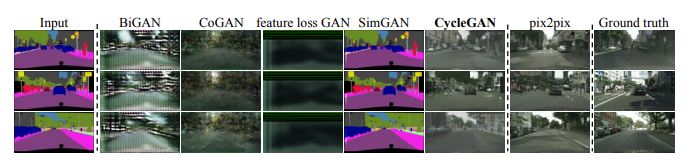
\includegraphics[width=\linewidth]{images/06_cycleGAN.PNG}
위 그림에서 주목할 점은 paired dataset에서 학습한 pix2pix에 비해서도 상당히 의미있는 결과를 cycleGAN이 도출해내었다는 것에 있다.
\newline  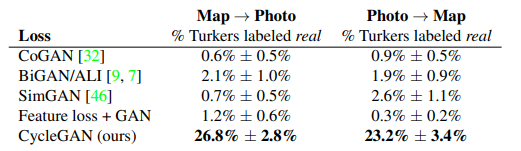
\includegraphics[width=6cm]{images/07_cycleGAN.PNG}
\newline 위의 결과는 사람이 얼마가 real인지 fake인지 판단한 값으로 꽤 높은 값을 얻었다는 것을 볼 수 있다.
\newline  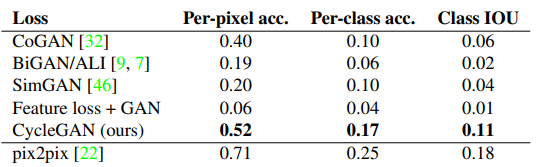
\includegraphics[width=6cm]{images/08_cycleGAN.PNG}
\newline 위의 결과는 FCN score을 계산한 것으로 다른 model에 비해 확연히 성능이 높고 paired dataset에서 학습한 pix2pix보다는 못하지만 꽤 의미있는 결과를 얻었다는 것을 볼 수 있다.
\newline  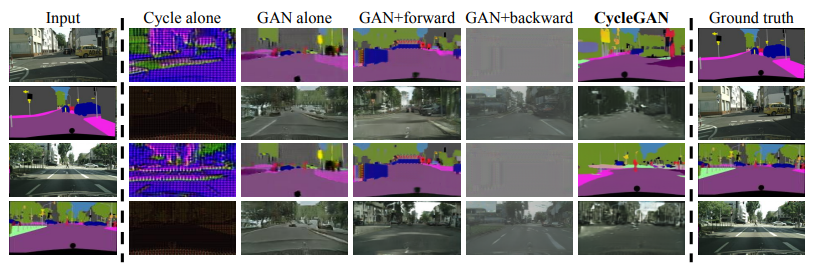
\includegraphics[width=\linewidth]{images/09_cycleGAN.PNG}
위의 그림은 cycleGAN의 손실 함수의 일부만을 사용한 결과이다. GAN 을 홀로 사용한거나 GAN+forward의 경우에는 mode collapse가 나타난다. mode collapse란 input이 다른데 만들어진 이미지의 경우에는
같아 input의 content을 유지하지 못한 결과가 나오는 오류이다. loss의 경우에는 모든 loss를 다 고려했을 때가 가장 보기에 groun truth와 비슷했다. 다만 FCN-score의 경우에는
GAN-forward cyle loss 만을 사용할 때가 가장 높기도 헀다. 이 저자들은 추가로 색깔을 유지하기 위한 $L_{identity}$을 제안하기도 한다. 왜냐하면 cycle GAN의 경우에는 content을 유지하는데에 쓰이기 때문이다.
그 식은 아래와 같다.
$$ L_{identity}(G,F) = E_{y~p_{data}(y)}[||G(y)-y||_1] + E_{x~p_{data}(x)}[||F(x)-x||_1]$$

\subsection{Conclusion}
\quad cycle GAN은 paired data에서 이미지를 생성하는 pix2pix를 unpaired dataset에서도 가능하게 만들어주었다는 것에 의미가 있다. 또한 loss에 cycle consistency를 추가하는 것으로 GAN의 단점을 보안했다는 점에서
구현 상으로도 크게 복잡하지 않다. 결과를 보면 paired dataset에서 학습한 pix2pix에 비해서는 성능이 떨어지지만 그래도 충분히 의미있는 결과를 얻는다.
단 cat이 dog로 바꾼다거나 하는 shape이 변해야 되는 task에서는 한계가 존재한다. 
\newpage
\bibliography{egbib}

\end{document}